\section{Rezolvarea numerică a ecuațiilor algebrice prin metoda înjumătățirii intervalului.}

În această lucrare de laborator va fi rezolvată determinarea rădăcinii unei ecuații de 
forma $f(x)=0$, dacă $f: x\subset \mathbb{R} \rightarrow \mathbb{R}$. \par
Când $f(x)$ este un polinom, sau poate fi adus, prin transformări corespunzătoare, la 
forma polinominală, ecuația se numește \textit{algebrică} (un exemplu concret ar servi 
ecuația $x^3+10x-9=0$). \par

\begin{figure}[H]
    \centering
    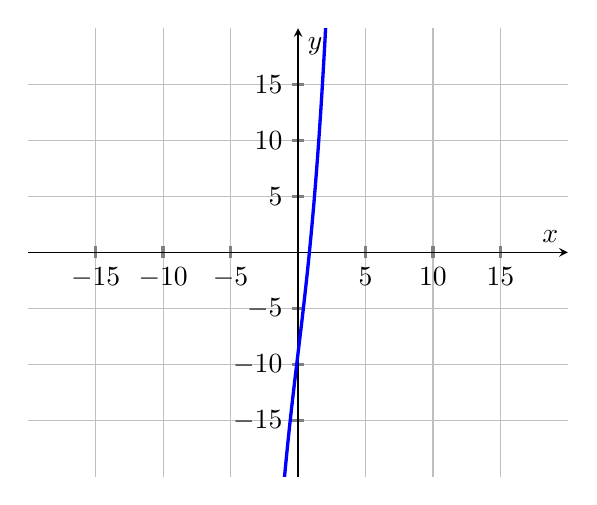
\begin{tikzpicture}
        \begin{axis}[
                axis lines=middle,
                grid=major,
                xmin=-20,
                xmax=20,
                ymin=-20,
                ymax=20,
                xlabel=$x$,
                ylabel=$y$,
                xtick={-15,-10,...,15},
                ytick={-15,-10,...,15},
                tick style={very thick}]
            \addplot[blue,very thick,samples=100] {x^3+10*x-9};
        \end{axis}
    \end{tikzpicture}
    \caption{Graficul funcției $x^3 + 10x - 9$.}
    \label{fig:grafic}
\end{figure}

La primă etapă, pentru rezolvarea ecuației, vom parcurge la \textit{separarea 
rădăcinilor} ecuației, pentru a preciza intervalul în care se gasește fiecare rădăcină 
reală a ecuației. \par

\textbf{Metoda bisecției} (sau metoda înjumătățirii intervalului) este una din cele mai simple 
metode iterative de rezolvare a unei ecuații neliniare care se bazează pe observația 
că funcția $f(x)$ are semne contrare la capetele intervalului $[a,b]$, în interiorul 
căreia se află soluția, adică $f(a) \cdot f(b) < 0$. \par

Se consideră deci ecuația de forma $f(x)=0, x \in [a,b]$, pentru care s-a separat în 
prealabil o soluție în intervalul $[a,b]$, adică $f(a) \cdot f(b) < 0$. Știind că 
funcția este continuă pe intervalul $[a,b]$, se cere să se determine soluția în cauză. \par

\begin{figure}[H]
    \centering
    \includestandalone{assets/bisection-plot}
    \caption{Demonstrarea grafică a metodei bisecției.}
    \label{fig:bisection-figure}
\end{figure}

Caracteristic metodei bisecției este că, pornind de la intervalul $[a,b]$, la fiecare 
pas se restrânge domeniul în care se caută soluția, prin înjumătățirea intervalului 
de la pasul anterior, până la atingerea preciziei dorite. \par

Aplicarea repetată a înjumătățirii intervalului de definiție a funcției, corespunzătoare 
unei ecuații a cărei soluție trebuie determinată, conduce la scăderea gradului de 
incertitudine al localizării soluției. \par

Această repetare se realizează în contextul probării unor condiții și a schimbării 
adaptate a capetelor intervalului. Algoritmul metodei înjumătățirii intervalului este 
descris în \textit{figura \ref{fig:diag}}.

\clearpage

\begin{wrapfigure}{r}{0.3\textwidth}
	\begin{tikzpicture}[node distance=1.8cm, scale=0.5, every node/.style={scale=0.5}]
		\node (start) [startstop] {Start};
		\node (in1) [io, below of=start] {$a, b, \varepsilon \in \mathbb{R}$};
		\node (dec1) [decision, below of=in1, yshift=-1.2cm] {\shortstack{$a > b$ \\ $f(a) \cdot f(b) > 0$}};
		\node (stop1) [startstop, right of=dec1, xshift=2.5cm]{End};
		\node (pro1) [process, below of=dec1, yshift=-1.8cm] {\shortstack{$c=\dfrac{a + b}{2}$ \\ $y_1 = f(a)$ \\ $y_2 = f(c)$}};
		\node (dec2) [decision, below of=pro1, yshift=-1.2cm] {$y_1 \cdot y_2 < 0$};
		\node (pro2a) [process, below of=dec2, yshift=-0.8cm] {$b = c$};
		\node (pro2b) [process, right of=dec2, xshift=2.5cm] {$a = c$};
		\node (dec3) [decision, below of=pro2a, yshift=-1cm] {$|a - b| \leqslant \varepsilon$};
		\node (out1) [io, below of=dec3, yshift=-1cm] {$a, b$};
		\node (stop2) [startstop, below of=out1, yshift=-0.2cm] {End};
		            
		\draw [arrow] (start) -- (in1);
		\draw [arrow] (in1) -- (dec1);
		\draw [arrow] (dec1) -- +(2,0) |- node[anchor=south] {Da} (stop1);
		\draw [arrow] (dec1) -- node[anchor=east] {Nu} (pro1);
		\draw [arrow] (pro1) -- (dec2);
		\draw [arrow] (dec2) -- node[anchor=east] {Da} (pro2a);
		\draw [arrow] (dec2) -- node[anchor=south] {Nu} (pro2b);
		\draw [arrow] (pro2a) -- (dec3);
		\draw [arrow] (pro2b) |- (dec3);
		\draw [arrow] (dec3) -- node[anchor=east] {Da} (out1);
		\draw [arrow] (dec3)  -- +(-2,0) |- node[anchor=south] {Nu} (pro1);
		\draw [arrow] (out1) -- (stop2);
	\end{tikzpicture}
	\caption{Diagrama metodei înjumătățirii intervalului.}
	\label{fig:diag}
\end{wrapfigure}

\clearpage

% http://users.utcluj.ro/~czumbil/documents/mn-cluj/MN_Cluj_Lab03_SuportTeoretic.pdf

\lstinputlisting[language={[Sharp]C}]{assets/BisectionMethod.cs} \par

\clearpage
